	
%%%%%%%%%%%%%%%%%%%%%%%%%%%%%%%%%%%%%%%%%%%%%%%%%%%%%%%%%%%%%%%%%%%%%
%% This is a (brief) model paper using the achemso class
%% The document class accepts keyval options, which should include
%% the target journal and optionally the manuscript type.
%%%%%%%%%%%%%%%%%%%%%%%%%%%%%%%%%%%%%%%%%%%%%%%%%%%%%%%%%%%%%%%%%%%%%
%\documentclass[journal=jpccck,manuscript=article,layout=twocolumn]{achemso}
\documentclass[journal=jpccck,manuscript=article]{achemso}

% UHe stuff
\def\EB{E_{\rm b}}

%%%%%%%%%%%%%%%%%%%%%%%%%%%%%%%%%%%%%%%%%%%%%%%%%%%%%%%%%%%%%%%%%%%%%
%% Place any additional packages needed here.  Only include packages
%% which are essential, to avoid problems later. Do NOT use any
%% packages which require e-TeX (for example etoolbox): the e-TeX
%% extensions are not currently available on the ACS conversion
%% servers.
%%%%%%%%%%%%%%%%%%%%%%%%%%%%%%%%%%%%%%%%%%%%%%%%%%%%%%%%%%%%%%%%%%%%%
\usepackage[version=3]{mhchem} % Formula subscripts using \ce{}
\usepackage[utf8]{inputenc}
\usepackage[T1]{fontenc}
\usepackage[english]{babel}
\usepackage{braket}
\usepackage{epsfig}
\usepackage{graphicx}
\usepackage{amsmath,amsfonts,amssymb}
\usepackage{dsfont}
\usepackage{booktabs}
\usepackage{units}
\usepackage{xcolor}
\usepackage{multirow}
\usepackage{tikz,pgfplots}
\usepackage{float} %force figure position

\usetikzlibrary{patterns,shadows,trees,calc}
\usepgfplotslibrary{units}

\pgfplotsset{compat=1.8}

%%%%%%%%%%%%%%%%%%%%%%%%%%%%%%%%%%%%%%%%%%%%%%%%%%%%%%%%%%%%%%%%%%%%%
%% If issues arise when submitting your manuscript, you may want to
%% un-comment the next line.  This provides information on the
%% version of every file you have used.
%%%%%%%%%%%%%%%%%%%%%%%%%%%%%%%%%%%%%%%%%%%%%%%%%%%%%%%%%%%%%%%%%%%%%
%%\listfiles

%%%%%%%%%%%%%%%%%%%%%%%%%%%%%%%%%%%%%%%%%%%%%%%%%%%%%%%%%%%%%%%%%%%%%
%% Place any additional macros here. Please use \newcommand* where
%% possible, and avoid layout-changing macros (which are not used
%% when typesetting).
%%%%%%%%%%%%%%%%%%%%%%%%%%%%%%%%%%%%%%%%%%%%%%%%%%%%%%%%%%%%%%%%%%%%%
%\newcommand*\mycommand[1]{\texttt{\emph{#1}}}
% Define some colours
\definecolor{diplom1}{rgb}{0.0 0.4 1.0}
\definecolor{diplom2}{rgb}{0.0 0.0 0.6}
\definecolor{diplom3}{RGB}{153,0,0} %unirot

%%%%%%%%%%%%%%%%%%%%%%%%%%%%%%%%%%%%%%%%%%%%%%%%%%%%%%%%%%%%%%%%%%%%%
%% Meta-data block
%% ---------------
%% Each author should be given as a separate \author command.
%%
%% Corresponding authors should have an e-mail given after the author
%% name as an \email command. Phone and fax numbers can be given
%% using \phone and \fax, respectively; this information is optional.
%%
%% The affiliation of authors is given after the authors; each
%% \affiliation command applies to all preceding authors not already
%% assigned an affiliation.
%%
%% The affiliation takes an option argument for the short name.  This
%% will typically be something like "University of Somewhere".
%%
%% The \altaffiliation macro should be used for new address, etc.
%% On the other hand, \alsoaffiliation is used on a per author basis
%% when authors are associated with multiple institutions.
%%%%%%%%%%%%%%%%%%%%%%%%%%%%%%%%%%%%%%%%%%%%%%%%%%%%%%%%%%%%%%%%%%%%%
\author{Elke Fasshauer}
\affiliation[UIT]{Centre for Theoretical and Computational Chemistry,
Department of Chemistry, University of Troms\o
-- The Arctic University of Norway, N-9037 Troms\o, Norway}
\email{elke.fasshauer@uit.no}
\author{Melanie Mucke}
\altaffiliation{Now at: Department of Physics and Astronomy, Uppsala University, Box 516, 75120 Uppsala, Sweden}
\author{Marko F\"orstel}
\altaffiliation{Now at: University of Hawai'i at Manoa, 2545 McCarthy Mall, 96816 HI Honolulu, USA}
\affiliation[IPP]{Max-Planck-Institute for Plasma Physics, Boltzmannstr. 2, 85748 Garching, Germany}
\author{...}
\author{Uwe Hergenhahn}
\affiliation[IOM]{Leibniz Institute of Surface Modification, Permoserstr. 15, 04318 Leipzig, Germany}
\alsoaffiliation[IPP HGW]{Max-Planck-Institute for Plasma Physics, Wendelsteinstr. 1, 14791 Greifswald, Germany}
\email{uwe.hergenhahn@ipp.mpg.de}
%\phone{+123 (0)123 4445556}
%\fax{+123 (0)123 4445557}
%\alsoaffiliation[Second University]
%{Department of Chemistry, Second University, Nearby Town}

%%%%%%%%%%%%%%%%%%%%%%%%%%%%%%%%%%%%%%%%%%%%%%%%%%%%%%%%%%%%%%%%%%%%%
%% The document title should be given as usual. Some journals require
%% a running title from the author: this should be supplied as an
%% optional argument to \title.
%%%%%%%%%%%%%%%%%%%%%%%%%%%%%%%%%%%%%%%%%%%%%%%%%%%%%%%%%%%%%%%%%%%%%
\title{One more attempt on ArXe}

%%%%%%%%%%%%%%%%%%%%%%%%%%%%%%%%%%%%%%%%%%%%%%%%%%%%%%%%%%%%%%%%%%%%%
%% Some journals require a list of abbreviations or keywords to be
%% supplied. These should be set up here, and will be printed after
%% the title and author information, if needed.
%%%%%%%%%%%%%%%%%%%%%%%%%%%%%%%%%%%%%%%%%%%%%%%%%%%%%%%%%%%%%%%%%%%%%
%\abbreviations{IR,NMR,UV}
%\keywords{American Chemical Society, \LaTeX}

%%%%%%%%%%%%%%%%%%%%%%%%%%%%%%%%%%%%%%%%%%%%%%%%%%%%%%%%%%%%%%%%%%%%%
%% The manuscript does not need to include \maketitle, which is
%% executed automatically.
%%%%%%%%%%%%%%%%%%%%%%%%%%%%%%%%%%%%%%%%%%%%%%%%%%%%%%%%%%%%%%%%%%%%%
\begin{document}

%%%%%%%%%%%%%%%%%%%%%%%%%%%%%%%%%%%%%%%%%%%%%%%%%%%%%%%%%%%%%%%%%%%%%
%% The "tocentry" environment can be used to create an entry for the
%% graphical table of contents. It is given here as some journals
%% require that it is printed as part of the abstract page. It will
%% be automatically moved as appropriate.
%%%%%%%%%%%%%%%%%%%%%%%%%%%%%%%%%%%%%%%%%%%%%%%%%%%%%%%%%%%%%%%%%%%%%
\begin{tocentry}

\begin{center}
 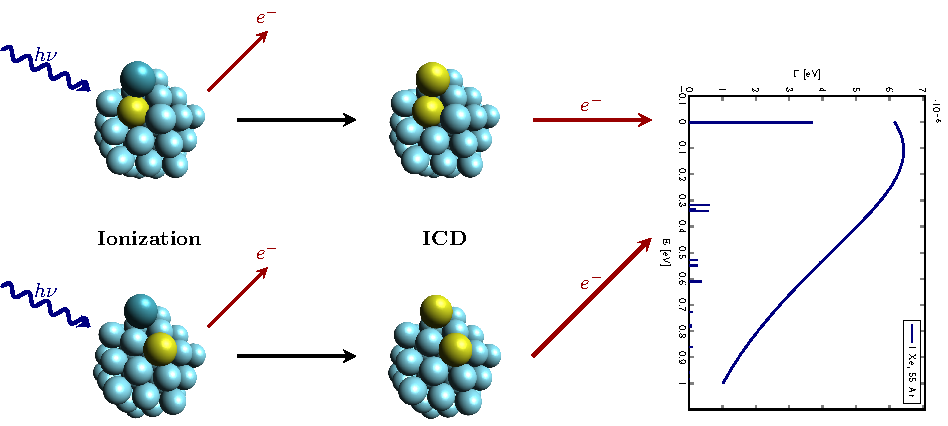
\includegraphics[height=3.5cm]{pics/front1.pdf}
\end{center}

%Some journals require a graphical entry for the Table of Contents.
%This should be laid out ``print ready'' so that the sizing of the
%text is correct.
%
%Inside the \texttt{tocentry} environment, the font used is Helvetica
%8\,pt, as required by \emph{Journal of the American Chemical
%Society}.
%
%The surrounding frame is 9\,cm by 3.5\,cm, which is the maximum
%permitted for  \emph{Journal of the American Chemical Society}
%graphical table of content entries. The box will not resize if the
%content is too big: instead it will overflow the edge of the box.
%
%This box and the associated title will always be printed on a
%separate page at the end of the document.

\end{tocentry}

%%%%%%%%%%%%%%%%%%%%%%%%%%%%%%%%%%%%%%%%%%%%%%%%%%%%%%%%%%%%%%%%%%%%%
%% The abstract environment will automatically gobble the contents
%% if an abstract is not used by the target journal.
%%%%%%%%%%%%%%%%%%%%%%%%%%%%%%%%%%%%%%%%%%%%%%%%%%%%%%%%%%%%%%%%%%%%%
\begin{abstract}
We report about autoionization channels of Ar inner valence ionized states in mixed ArXe clusters. 
The mixed clusters were produced by supersonic coexpansion of the two gases.
Clusters with a range of sizes and compositions were probed. 
The Xe content in the clusters was varied between 10 and 53\,\%. 
Our experimental data obtained by electron, electron coincidence spectroscopy are compared to theoretical simulations for representative cluster structures.
The combined experimental and theoretical data show that the autoionization of Ar 3s$^{-1}$ in ArXe is dominated by Interatomic Coulombic Decay (ICD) to Xe atoms in the second and higher coordination shells of the originally excited atom.
Electron Transfer Mediated Decay (ETMD3) is energetically allowed as well for
most cluster structures. It is even dominant for some of the cluster
structures, but has less intensity in the experimental spectra. We therefore
conclude that 
cluster structures with either a clear seggregation between Ar and Xe fractions, e.g. Xe core, Ar shell systems, or with few Xe atoms singled out in surface sites
are favoured.
These structures differ significantly from the majority of calculated minimum
energy structures for ArXe systems of 38 atoms, which might show that the latter structures are not realized in supersonic expansion.

We show experimentally that the relaxation of Ar inner valence states by ICD and ETMD together has an efficiency of unity, within the experimental accuracy, for all clusters expect those with the lowest Xe content.
\end{abstract}


%%%%%%%%%%%%%%%%%%%%%%%%%%%%%%%%%%%%%%%%%%%%%%%%%%%%%%%%%%%%%%%%%%%%%
%% Start the main part of the manuscript here.
%%%%%%%%%%%%%%%%%%%%%%%%%%%%%%%%%%%%%%%%%%%%%%%%%%%%%%%%%%%%%%%%%%%%%
%%%%%%%%%%%%%%%%%%%%%%%%%%%%%%%%%%%%%%%%%%%%%%%%%%%%%%%%%%%%%%%%%%%%%
%% Start the main part of the manuscript here.
%%%%%%%%%%%%%%%%%%%%%%%%%%%%%%%%%%%%%%%%%%%%%%%%%%%%%%%%%%%%%%%%%%%%%
\section{Introduction}
%
Electron spectroscopy can make important contributions to the 
research on composition and structure of free nanoparticles.\cite{
jpcc} Besides photoionization, free electrons emerging from 
nanoparticles can also be produced by the relaxation of 
electronically excited states. One such process, which is of 
particular relevance in weakly bonded systems, is the 
Interatomic or Intermolecular Coulombic Decay (ICD).\cite{
cederbaum} In ICD, an electronic excitation decays by energy 
transfer to one of its neighboring atoms or molecules, thus 
releasing a free electron from the latter site. ICD is an 
important relaxation channel e.g. for inner-valence holes in 
atoms, and also for core level vacancies e.g. in \ce{H2O}
, where it competes with Auger decay.\cite{slavicek}

By definition, ICD is particularly sensitive to the chemical 
environment of the atom or molecule in which the primary 
excitation has taken place. We suggest that this property of ICD 
decay spectra can be used to derive information on a nanoparticle 
or a solvation system. 
The term excitation is used here in a broader sense---in the
systems we consider in this work, ICD occurs from an excited, singly 
charged Ar state created by photoionization.
In other systems, ICD was also observed from neutral excited
states and states with more than one vacancy.

We report here about studies 
in which we produced heterogeneous clusters of the noble gases Ar 
and Xe with different sizes, and compositions ranging from a few 
Xe dopant atoms in an Ar matrix to clusters containing an equal 
amount of both species. By the use of electron-electron 
coincidence spectroscopy and of theoretical simulations on 
prototypical systems we show how the radiationless decay spectrum 
of Ar inner valence (3s) ionized states connects to the structure 
of the clusters.

Intermolecular Coulombic Decay initially was predicted from 
theoretical considerations of the energy levels in singly vs.\  
doubly ionized, and doubly vs.\ triply ionized, hydrogen bonded 
clusters.\cite{cederbaum} First experimental work some years 
later used Ne clusters,\cite{marburger,jahnkenedimer} but quickly 
was followed by demonstrations of ICD in a diverse range of other 
systems. Experimental and theoretical progress has been reviewed.
\cite{hergenhahn_review, averbukh_review, jahnke_review} ICD 
proceeds by an initial ionization producing an ion in an excited 
state, followed by a transfer of energy to a neighbouring site, 
and an electron emission process therefrom. The final state contains 
two positive charges; one at the original site of ionization, and a second
one at another atom or molecule. 

Soon after, related 
autoionization processes were discovered that are governed by a
charge transfer instead of an energy transfer. 
These were termed `Electron Transfer Mediated Decay' 
 (ETMD),\cite{zobeley,mueller,sakai,foerstel} for transitions in 
 which the originally excited site is neutralized by the decay 
and `exchange ICD' for charge transfer contributions to the 
normal ICD amplitude.\cite{santrarev,jahnkesat}

We find that both energy and charge transfer induced 
autoionization play a role in Ar-Xe, and will detail the 
relevant processes below. The notion of ICD requires that the 
electronic orbitals of the two sites can be distinguished, which 
typically is the case in weakly bonded systems, held together by 
hydrogen bonds or van-der-Waals bonds. In the case of strong
(covalent or metallic) bonding, it is impossible to make a
distinction between ICD and Auger decay.\cite{hergenhahn_review}

Rare gas clusters are suitable prototype systems for studies of
ICD, as they can readily be produced by supersonic 
expansion through a cooled nozzle. 
The size of the clusters can be changed by varying the expansion parameters.
The formation of heterogeneous rare gas clusters by coexpansion of a gas mixture cannot {\it a priori} be taken for granted, but was experimentally shown for most combinations of two rare gases, when suitable mixing ratios and expansion parameters are used (see references throughout this article).

First experiments on ICD in heterogeneous systems used Ne-Ar 
clusters.\cite{barthnear} Those were followed by studies of 
ICD-like inner-shell decays in aqueous solution.\cite{aziz,pokapanich,pokapanich2011}
Pioneering work also showed the 
potential for studies of the interface between a substrate and an 
adsorbate by ICD.\cite{grieves} More detailed work on Ne-Ar 
clusters was recently presented by some of the authors \cite{fasshauer2014}
showing that an analysis of the ICD spectra
allowed to decide between structural alternatives, for which the
photoelectron data were indiscriminate.
For this system, a detailed account of the
photoelectron spectra with respect to structural features of the 
mixed clusters is also available.\cite{lundwall}

Several experimental techniques have been used for the study of mixed Ar-Xe clusters, most notably fluorescence spectroscopy, electron diffraction and photoelectron spectroscopy. 
Early work focussed on the fluorescence of a single Xe atom 
embedded in an Ar cluster.\cite{lengenprl}
%Different sites of the dopant atom (on top of a surface, 
%integrated in an Ar surface, inside the cluster) were 
%distinguished by three separate bands in the fluorescence yield 
%recorded as a function of excitation wavelength.\cite{goldberg} 
Increasing the Xe concentration in the expansion lead to the formation of \ce{Xe2} and larger Xe complexes inside the clusters.\cite{lengen} 
With increasing Xe content, the formation of Xe-core, Ar-shell systems with a sharp interface between the two species was shown in photoionization experiments.\cite{tchaplyguine,hoener}
This finding was confirmed by electron diffraction.\cite{Danylchenko,Danylchenko07} 
Always, the observed Xe content in the clusters is higher than the Xe content in the expanding gas mixture, as Xe can be condensed much easier than Ar.\cite{hoener,Danylchenko07}
%A complementary study used photoelectron-photoion coincidence of
%large Ar-Xe clusters, and found that after inner shell (Xe 4d, Ar 2p)
%photoionization significant charge transfer between both species
%occurs before the mass spectroscopic final state is reached.\cite{berrah}
%
More recently, photoelectron spectra of 
small Ar-Xe clusters were analyzed, adding to the findings in 
earlier work.\cite{lindblad} We will discuss this paper in 
connection with our results below. 
For completeness, we mention that Ar-Xe complexes can also be produced by passing clusters from a neat Ar expansion through a zone filled with Xe gas (`pick-up').\cite{pietrowski}
Clusters produced such can structurally be quite different from those produced by coexpansion.\cite{lindbladpccp}

A number of theoretical works on Ar-Xe clusters aimed at the prediction of minimum energy structures. 
Most recently, these converged to structures which have the Xe atoms mainly in the interior.\cite{marques} 
Xe was also found to diffuse into the interior of Ar clusters in molecular dynamics simulations after pick-up.\cite{Vach_1999} 
The electronic energy levels of very small Ar-Xe clusters were calculated in ref \citenum{fasshauer} and the secondary electron spectra were simulated for
model structures of one argon atom placed on a xenon surface \cite{Fasshauer13}.
Interestingly, it was found that Ar 3s$^{-1}$ is stable 
against autoionization in an ArXe dimer, but is destabilized by 
adding further Xe atoms, or an Ar solvation shell, to the system, thereby allowing
for combinations of argon and xenon atoms with larger interatomic distances. 
Again, we will detail these results in conjunction with our 
current work.

The plan of our paper is as follows: We firstly delineate our experimental and theoretical methods. 
Calculations were done for a number of model structures which were systematically varied, and are described in the following section.
After that, we describe and discuss our theoretical results for the autoionization spectra of the model clusters.
Experimental results are then shown and possible conclusions from comparing them to the calculations are given.
Details on the experimental technique, and calculated spectra for a wider range of structures are given as Supporting Information.

%\begin{figure}
%  As well as the standard float types \texttt{table}\\
%  and \texttt{figure}, the class also recognises\\
%  \texttt{scheme}, \texttt{chart} and \texttt{graph}.
%  \caption{An example figure}
%  \label{fgr:example}
%\end{figure}

%\begin{table}
%  \caption{An example table}
%  \label{tbl:example}
%  \begin{tabular}{ll}
%    \hline
%    Header one  & Header two  \\
%    \hline
%    Entry one   & Entry two   \\
%    Entry three & Entry four  \\
%    Entry five  & Entry five  \\
%    Entry seven & Entry eight \\
%    \hline
%  \end{tabular}
%\end{table}


\section{Experimental}
%
\begin{table}
\caption{
Expansion parameters used for cluster production. Here, Xe$_{\rm in}$ is the molar fraction of Xe in the gas mixture before the expansion, $T$ is the nozzle temperature, and $p$ the stagnation pressure. Experiments were done with $d = 80~\mu$m (first two sections) and $d = 100~\mu$m (bottom section) conical nozzles of 15$^\circ$ half opening angle. For the mixed clusters, $\langle N_{\rm Ar} \rangle$ and $\langle N_{\rm Xe} \rangle$ refer to cluster sizes arrived at by an expansion of the respective pure gases at the given conditions. These values are calculated as in ref.\ \protect\citenum{hagena1981}. Due to the much lower freezing point of Ar, we basically have an Ar seeded expansion of Xe gas. We therefore expect actual cluster sizes in-between the two limiting values given. Inaccuracies in the calculation of $\langle N\rangle$ due to fluctuations of the input parameters are less than 6\,\%. This figure does not include systematic errors of the empirical model used.
}
\label{tab:cluster}

\begin{tabular}{l c c c c r r}
%
\toprule
  \multicolumn{2}{r}{size label}  &  Xe$_{\rm in}$ (\%)  &  $T$ (K)  &  $p$ (bar) & $\langle N_{\rm Ar} \rangle$ & $\langle N_{\rm Xe} \rangle$ \\
%
\midrule
% Ar, from Marko 
Ar & (1) & --- &  96.5  & 0.35  &  42  &  --- \\
% Ar, from Marko 
Ar & (2) & --- &  96.5  & 0.67  & 190  &  --- \\
% 1103 676, 679
ArXe & S & 1.2 &  174   & 0.32  &   4  &   62 \\
% 1103 670
ArXe & M & 1.2 &  174   & 0.49  &  10  &  168 \\
% 1103 671
ArXe & L & 1.2 &  174   & 0.68  &  21  &  362 \\
% 1103 663
ArXe & S & 3.0 &  172   & 0.28  &   3  &   48 \\
% 1103 640
ArXe & M & 5.0 &  171   & 0.51  &  12  &  202 \\
% 0506 382, Keller offset ber?cksichtigt
Xe &  & 100 & 183.5  & 0.68  & ---  &  517 \\     
\midrule
% 1103 653
ArXe & M & 3.0 &  172   & 0.51  &  11  &  196 \\
% 1103 658
ArXe & L & 3.0 &  172   & 0.68  &  22  &  385 \\
% 1103 630
ArXe & S  & 5.0 &  167   & 0.37  &   6  &  108 \\
% 1103 629
ArXe & L  & 5.0 &  167   & 0.68  &  26  &  451 \\
\midrule
% 1004 867 (32 eV)
ArXe & XL & 2.5 &  154   & 2.12  &  920 & 15760\\
% 1004 868
%868 & & 2.5 &  158   & 1.50  &  355 &  6090\\
% 1004 886 (17 eV)
%886 &  & 2.5 &  161   & 2.41  &  980 & 16770\\
% 1004 858
%858 &  & 5.0 &  149   & 2.50  & 1620 & 27700\\
%
\bottomrule
\end{tabular}
\end{table}
%
%
The apparatus used for the experiments consists of a supersonic molecular jet with a cooled nozzle, and a magnetic bottle spectrometer, which detects photoelectrons and secondary electrons produced after ionization with synchrotron radiation.\cite{arion} 
% Leave this citation in place to avoid Latex error
A detailed description can be found in Ref. \citenum{arion}, and here we focus on details specific for the current experiment. Commercial Ar and Xe gas was used. 
Separate containers for the two gases were filled up to pressures suitable for producing a certain mixing ratio. The gases were then allowed to mix before the expansion. 
Expansion parameters and mean cluster sizes, according to an empirical model, are given in Tab.\ \ref{tab:cluster}. 
We note that currently no empirical model for cluster sizes in a heterogeneous gas expansion exists. 
We therefore can only give the mean size for a pure jet of one or the other gas at the given conditions. 

The expansion chamber for the supersonic jet is separated from the interaction chamber by a non-magnetic, conical skimmer with a diameter 1~mm opening (Beam Dynamics). 
At few cm distance behind the skimmer, the cluster jet was crossed by synchrotron radiation from the BESSY electron storage ring at Helmholtz-Zentrum Berlin. 
Electrons were detected by a short `magnetic bottle' time-of-flight spectrometer, that has been described earlier.\cite{mucke_review} 
Data were recorded in two different beamtimes at the UE112-PGM-1 (small and medium sized clusters, first two sections in Tab.\ \ref{tab:cluster}) and at the TGM-4 beamline (large clusters, last section in Tab.\ \ref{tab:cluster}). 
Linearly, horizontally polarized radiation was used. 
The storage ring was operated in single bunch conditions.




\section{Theoretical Approach}
%
We are interested in describing the electron emission spectra of excited states in clusters, that where measured by the electron-electron coincidence method in our experiments. 
In our theoretical description, these will be composed of multiple transitions, each characterized by a kinetic energy $E_{\rm sec}$ of the secondary electrons, and the intensity of the peak.
The latter is proportional to the probability of the decay, represented here by the decay width $\Gamma_\beta = \hbar/\tau_\beta$, where $\tau_\beta$ is the lifetime due to the respective transition.
The total decay width $\Gamma$ is the sum of all partial $\Gamma_\beta$.
In case of noble gas clusters with a given geometrical structure, three aspects have to be taken into account:
different decay mechanisms, the contribution of different cluster sites to the respective decay, and the existence of different decay channels within each decay mechanism.
At the current stage of development we have to neglect the nuclear dynamics, which
additionally might play an important role.

This means, for the evaluation of the decay width we are dealing with a sum over three different indices: 
For a given structure it is most convenient to
start with a decomposition of the system into interaction partners of
the different decay mechanisms, i.e. pairs (combination of two atoms regardless
of their internuclear distance) for the ICD and triples (combinations of three atoms)
for the ETMD.
{\em Q: Doubles for ETMD(2) and triples for ETMD(3) ?! Do we make this distinction here?}
These atoms do not necessarily need to form bonds between each other or
even be close, but they are characterized according to fixed internal
coordinates. 
Each pair and each triple leads to a decay spectrum that can be described by the energy of the secondary electron and the decay width, and which is in first order of approximation independent of other atoms present in the cluster.
In the following, this approach will be called model of pairs and triples.


%Decomposing every system into pairs and triples of atoms is a very useful
%first order approximation to both the investigation of energies and
%decay widths of a larger system. Pairs and triples are combinations of
%two and three atoms, respectively.

In order to determine, whether a channel $\beta$ for a given geometry and decay
mechanism is open, i.e., whether it is in accordance with energy conservation,
knowledge of the energies of the initial and the final states, $E_{\rm in}$ and $E_{\rm fin}$, of
the corresponding processes are necessary.
If the channel
is open, the excess energy is carried away by the emitted electron
in form of its kinetic energy $E_{\rm sec}$. These energies in the model
of pairs and triples can be approximated by

\begin{align}
 E_{\rm in}        &= SIP(X_{\rm in}) \label{equation:E_in}\\
 E_{\rm fin}^\beta &= SIP(X_{D}^\beta) + SIP(X_{E}^\beta) + \frac 1d
           \label{equation:E_fin}\\
 E_{\rm sec}^\beta &= E_{\rm in}^\beta - E_{\rm fin}^\beta \label{equation:E_sec}
\end{align}
where $X_{\rm in}$ denotes the initially ionized atom and
$X_{D}$ and $X_{E}$ describe the electron donating atom and electron
emitting atom, respectively.
$\beta$ denotes the decay channel characterized by the quantum numbers of the ionized atoms in the pairs and triples, $SIP(X^\beta)$ the single ionization potential of vacancy $\beta$ in atom $X$ and $d$ the interatomic distance between the atoms $X_{D}$ and $X_{E}$. 
Atomic units are used.
The initially ionized atom $X_{\rm in}$ can
coincide with one or both of
the final state atoms
$X_{D}$ and $X_{E}$.
The distribution of the vacancies over the different
atoms determines the kind of electronic decay process at hand. Hence, in an
Auger process all three atoms coincide, for an ICD process $X_{\rm in}$
coincides with $X_{D}$ and for an {ETMD}3 process
all ionized states are located on different atoms.

\begin{figure}[h]
 \centering
 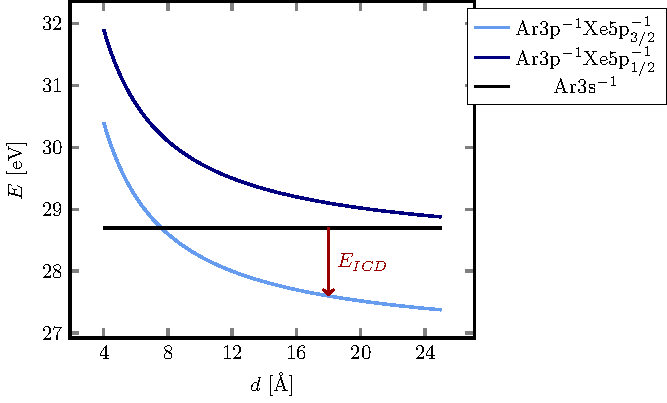
\includegraphics[width=8.5cm]{pics/channel_open_ICD.pdf}
 \caption{Initial (black trace) and final state energies (blue traces) 
          for ICD in ArXe pairs as a function of 
          internuclear distance, using the experimental ionization potentials given
          in Table \ref{}. For distances larger than the channel opening
          distance the ICD channel is open.}
 \label{figure:channel_open_ICD}
\end{figure}

The electron emitted by autoionization has the kinetic energy $E_{\rm sec}$. 
If the calculated value of $E_{\rm sec}$ is negative,
the final state energy is higher than the initial state energy and the        
process is energetically not accessible. Hence, the corresponding channel     
is closed, as shown in Figure \ref{figure:channel_open_ICD}. Related to
the opening of each channel is an internuclear distance which we will call 
\emph{channel opening distance} in the following.
                                                               
This {\latin ad hoc} approach allows to easily correct for energetic shifts of ionization potentials as observed in larger clusters by adding experimentally or theoretically determined energy shifts $\Delta E(X_{A}^{\beta})$ for a given vacancy $A={\rm in},D,E$ and channel $\beta$. This yields the working expression for the kinetic energy of the secondary electron:

\begin{equation}
 E_{\rm sec}^\beta = SIP(X_{\rm in}) + \Delta E (X_{\rm in})
               - SIP(X_{D}^\beta) - \Delta E (X_{D}^\beta)
               - SIP(X_{E}^\beta) - \Delta E (X_{E}^\beta)
               - \frac 1d .
\end{equation}

The total decay width $\Gamma$ is given by the sum over the decay widths
of all decay mechanisms. In case of the ArXe clusters we only consider
ICD and ETMD:

\begin{equation}
 \Gamma = \Gamma_{\rm ICD} + \Gamma_{\rm ETMD} .
\end{equation}

These are given by the sum over the decay widths of all pairs $i$ for the
ICD and all triples $j$ for the ETMD(3), respectively, and over all channels $\beta$:
%
\begin{align}
 \Gamma_{\rm ICD}  &= \sum\limits_{i,\beta} N_{{\rm ICD},i}  \, \Gamma_{{\rm ICD},i,\beta},\\
 \Gamma_{\rm ETMD} &= \sum\limits_{j,\beta} N_{{\rm ETMD},j} \, \Gamma_{{\rm ETMD},j,\beta}.
\end{align}
Here, $N_{{\rm ICD},i}$ and $N_{{\rm ETMD},j}$ denote the number of geometrically
equal pairs and triples in a given cluster structure. The total number of pairs
reads
$N_{{\rm ICD}} = N_{\rm in} \cdot N_{D/E} = N_{\rm Ar} \cdot N_{\rm Xe}
 = \sum\limits_i N_{{\rm ICD},i}$ and the number of triples is
$N_{{\rm ETMD}} = N_{\rm in} \cdot N_{D/E} (N_{D/E} - 1) = N_{\rm Ar} \cdot N_{\rm Xe} (N_{\rm Xe} - 1)
 = \sum\limits_j N_{{\rm ETMD},j}$.
The numbers of geometrically equivalent pairs $N_{{\rm ICD},i}$ and triples $N_{{\rm ETMD},j}$
strongly depend on the structure of the cluster. From these relationships
it can be seen that a higher xenon content in the cluster statistically
favours the ETMD(3) over the ICD.

In previous work \cite{Fasshauer13,Fasshauer_thesis} we have shown that
the decay width for a single pair or triple for a distinct channel $\beta$
following Wentzel \cite{Wentzel27}, Feshbach\cite{Feshbach58,Feshbach62}
and Fano,\cite{Fano61}
%
\begin{equation}
 \Gamma_{\beta}(E_{\rm res}) = 2\pi \left|
                           \braket{\Phi_{\rm in}| H_f |\chi_{\beta}}
                           \right|^2,
\end{equation}
%
can be approximated by its asymptotic behaviour
%
\begin{equation}
 \Gamma_{{\rm ICD},i,\beta} = (2J_{\rm in}+1)\, \frac{3c^4}{8\pi}\,
                        \sum\limits_{M_{in}'}
                        \left| \left(
                        \begin{array}{ccc}
                        J_A'  & 1        & J_A\\
                        -M_A' & M_A'-M_A & M_A
                        \end{array}\right) \right|^2
                        \frac{\sigma^{(X_E)}(\omega_{vp,\beta})}
                        {R_i^6 \, \omega_{vp,\beta}^4 \tau_{in,\beta}}
\end{equation}
%
and
%
\begin{equation}
 \Gamma_{{\rm ETMD},j,\beta} = \frac{c}{2\pi} \sum\limits_{m,k,M_{in}',D}
                        \frac{a_{m,k} \Theta_{m,k}(\alpha_j) \sigma^{(X_E)}(\omega_{vp,\beta})
                              \tilde{D}_{m,j,\beta}(M_{in,D},M_{in,D'})}
                         {R_j^6 \omega_{vp,\beta}}
\end{equation}
%
depending on constants ($a_{m,k}=4,2$)
as well as experimental properties
of atoms, like the ionization cross sections
$\sigma^{(X_E)}(\omega_{vp,\beta})$, radiative lifetimes of the initially
ionized state $\tau_{in,\beta}$ and the excess energy transferred to the
emitting atom (the energy of the virtual photon) $\omega_{vp,\beta}$
and calculated dipole transition moments $\tilde{D}_{m,j,\beta}$, only.
Here, $\Theta_{m,k}(\alpha_j)$ is a function depending on the angle $\alpha_j$
of the triple, the direction of the dipole
transition moment $m$ and an additional index $k$
(compare Ref. \cite{Fasshauer13}).

In this work we evaluate the secondary energies and decay widths with
the program HARDRoC \cite{HARDRoC,fasshauer2014} using the
experimental ionization energies of Table \ref{}
and data from the literature given in Tables \ref{} and \ref{}.
This choice is identical to the one made in Reference \cite{Fasshauer13}.

\section{Cluster Structures}

\section{Theoretical Results}

The geometrical properties as well as the total ICD and ETMD decay widths
of the investigated structures are shown in Table \ref{table:theo_gammas}.
It is important to remember that the first ICD channel opens at a
channel opening distance of \unit[7.58]{\AA}. Therefore, small
clusters in which none of the possible Ar-Xe pairs in larger than
these \unit[7.58]{\AA}, no ICD can take place. Also, two xenon atoms are
required for an ETMD3 and hence the ETMD3 has to be excluded from
the possible decay mechanism in clusters with only one xenon atom.
Because secondary electrons are observed in the experimental spectra
we exclude all structures without any signal from our further
discussions.

\begin{table}[h]
\centering
\caption{Properties of simulated clusters.}
\begin{tabular}{lrrrccc}
\toprule
name                 & Xe atoms & Ar atoms & Xe \% &   ICD                &  ETMD                & $\Gamma_{ICD,ETMD}$\\
\midrule
ArXe\_2\_1atom       &      1   &     12   &  7.7  &      0.0             &  0.0                 &     0.0            \\
ArXe\_3\_1atom       &      1   &     54   &  1.8  &      0.0             &  0.0                 &     0.0            \\ 
ArXe\_3\_2atom       &      2   &     53   &  3.6  & 3.346$\cdot 10^{-6}$ & 1.666$\cdot 10^{-5}$ & 2.006$\cdot 10^{-5}$ \\
ArXe\_8\_1layer      &   1415   &    642   & 68.8  & 7.039$\cdot 10^{-4}$ & 2.573$\cdot 10^{-4}$ & 9.612$\cdot 10^{-4}$ \\
\midrule
XeAr\_2\_surface     &      1   &     13   &  7.1  & 7.922$\cdot 10^{-5}$ & 0.0                  & 7.922$\cdot 10^{-5}$ \\
XeAr\_2\_edge        &      1   &     13   &  7.1  & 1.320$\cdot 10^{-6}$ & 0.0                  & 1.320$\cdot 10^{-6}$ \\
XeAr\_2\_vertex      &      1   &     13   &  7.1  & 5.013$\cdot 10^{-6}$ & 0.0                  & 5.013$\cdot 10^{-6}$ \\
XeAr\_2\_2top        &      2   &     13   & 13.3  & 1.011$\cdot 10^{-5}$ & 1.513$\cdot 10^{-5}$ & 2.523$\cdot 10^{-5}$ \\
XeAr\_2\_2midtop     &      2   &     13   & 13.3  & 1.588$\cdot 10^{-5}$ & 7.686$\cdot 10^{-7}$ & 1.665$\cdot 10^{-5}$ \\
XeAr\_2\_2endtop     &      2   &     13   & 13.3  & 1.587$\cdot 10^{-5}$ & 1.772$\cdot 10^{-7}$ & 1.605$\cdot 10^{-5}$ \\
XeAr\_3\_surface     &      1   &     55   &  1.8  & 6.371$\cdot 10^{-6}$ & 0.0                  & 6.371$\cdot 10^{-6}$ \\
XeAr\_3\_edge        &      1   &     55   &  1.8  & 4.791$\cdot 10^{-6}$ & 0.0                  & 4.791$\cdot 10^{-6}$ \\
XeAr\_3\_vertex      &      1   &     55   &  1.8  & 2.701$\cdot 10^{-6}$ & 0.0                  & 2.701$\cdot 10^{-6}$ \\
XeAr\_3\_edge\_in    &      1   &     54   &  1.8  & 7.708$\cdot 10^{-6}$ & 0.0                  & 7.708$\cdot 10^{-6}$ \\
XeAr\_3\_vertex\_in  &      1   &     54   &  1.8  & 5.258$\cdot 10^{-6}$ & 0.0                  & 5.258$\cdot 10^{-6}$ \\
XeAr\_3\_2in         &      2   &     53   &  3.6  & 1.166$\cdot 10^{-5}$ & 5.453$\cdot 10^{-6}$ & 1.711$\cdot 10^{-5}$ \\
XeAr\_3\_6in         &      6   &     49   & 10.9  & 3.746$\cdot 10^{-5}$ & 4.050$\cdot 10^{-5}$ & 7.796$\cdot 10^{-5}$ \\
XeAr\_3\_6\_scat     &      6   &     49   & 10.9  & 2.923$\cdot 10^{-5}$ & 6.737$\cdot 10^{-5}$ & 9.660$\cdot 10^{-5}$ \\
\bottomrule
\end{tabular}
\label{table:theo_gammas}
\end{table}

In the investigated structures several different aspects have to be
taken into account which we will discuss separately if possible
on selected structures.

Firstly, we consider two different argon core sizes one consisting
of 13 and one consisting of 55 atoms with one xenon atom on one of
the surfaces (see Figure \ref{figure:cluster_3_overview} Panel a)
for the 55 atom core). The simulated secondary electron spectra are
shown in Figure \ref{figure:surf} Panel 1.

\begin{figure}[ht]
 \centering
 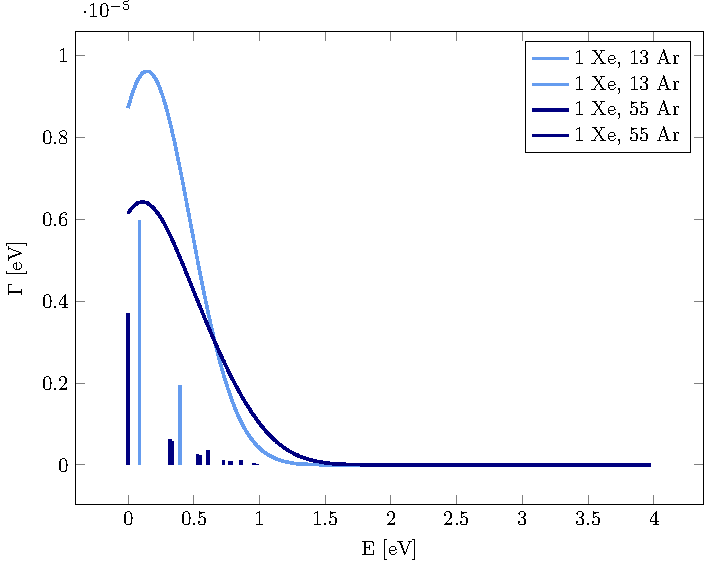
\includegraphics[width=8.5cm]{pics/surf.pdf}\\
 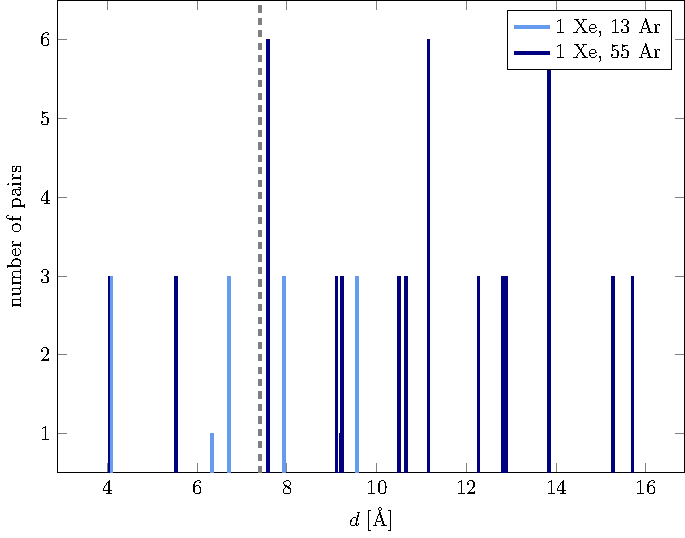
\includegraphics[width=8.5cm]{pics/R_comp.pdf}
 \caption{Panel 1: Simulated electron-electron coincidence spectra
          for argon clusters
          consisting of 13 and 55 atoms with on additional xenon atom residing
          on top of one of the argon surfaces.\\
          Panel 2: Distribution of Ar-Xe distances $d$ in the studied ArXe
          clusters. The ICD channels open at \unit[7.58]{\AA} and
          \unit[36.00]{\AA}, respectively. Hence only pairs at longer interatomic
          distances than the gray line contribute to the coincidence spectra.
          The distance distribution of the larger cluster contains larger
          distances which correspond to peaks at higher kinetic energies of
          the ICD electron in the coincidence spectra (Panel 1).}
 \label{figure:surf}
\end{figure}

Because the structures have only one xenon atom ETMD3 is not possible and
ICD only is to be expected. Both spectra show several smaller peaks which
are convoluted into one single peak with a maximum at
approximately \unit[0.2]{eV}. In comparison to the 13 argon atoms core
spectrum the 55 argon atoms core spectrum shows
signals at higher energies of the secondary electron. These features
can be explained by analysis of the Ar-Xe distances in the clusters shown
in Figure \ref{figure:surf} Panel 2. Every different atom pair distance
yields in a different energy of the secondary electron and only pairs
with a distance of larger than the channel opening distance
(dashed, gray line) will contribute
to the spectrum. The larger the interatomic distance is, the higher is the
kinetic energy of the secondary electron for a given channel.
Since the 55 argon atom core cluster is larger and therefore
has Ar-Xe pairs with larger distances its spectrum has signals at higher
energies as well.
This effect holds for all clusters.


For clusters with more than one xenon atom the ETMD3 channel is possible
as well. Depending on the positions of the relative positions of the xenon
atoms in or on the cluster the spectra are expected to be different.
As an example we therefore discuss the secondary electron spectra of the
clusters with an 13 argon atoms core and two xenon atoms on different
surfaces illustrated in Figure \ref{figure:cluster_2_overview} shown in Figure
\ref{figure:2tops}. In these the xenon content is \unit[13.3]{\%} and therefore
close to the experimental ones of \unit[10-12]{\%} for the low xenon pressure.

\begin{figure}[h]
 \centering
 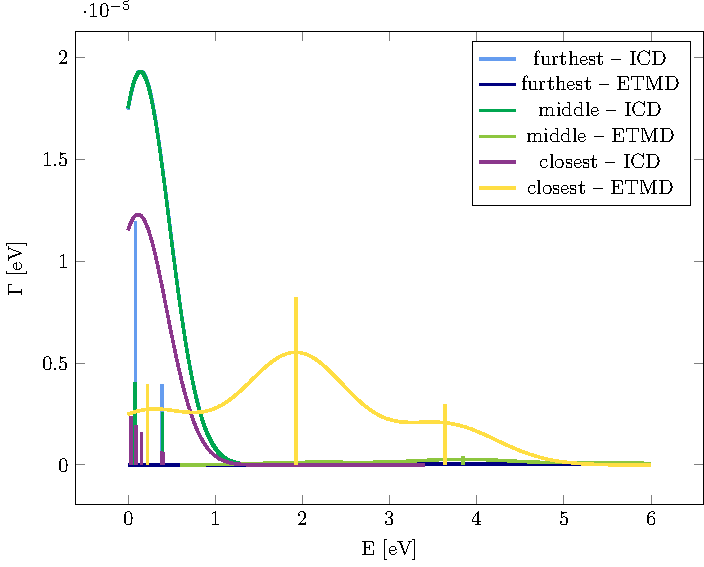
\includegraphics[width=8.5cm]{pics/2tops.pdf}
 \caption{Simulated coincidence spectra of argon clusters consisting of 13
          argon atoms with 2 additional xenon atoms on top of two different
          argon surfaces. The ICD and ETMD spectra are shown for all three
          different relative positionings of the two xenon atoms. In case of
          the two xenon atoms being close to each other, an ETMD process is
          clearly visible. In the other two cases the spectra are dominated by
          the corresponding ICD spectrum.}
 \label{figure:2tops}
\end{figure}

In all three cases both ICD and ETMD3 are energetically allowed and the ICD
spectra are either identical or at least very similar consisting of one
convoluted peak at approximately \unit[0.2]{eV}. However, the ETMD3 spectra
are very sensitive to the relative positioning of the two xenon atoms.
Two aspects have to be taken into account: an energy shift of the peak due
to different charge distances in the final state (i.e. the interatomic Xe-Xe
distance) and the different decay widths decreasing with $\frac{1}{R^6}$
between the electron transfer unit and the finally ionized xenon atom.
The larger the distance between the xenon atoms is, the lower are the energies
of the secondary electrons and the higher are the decay widths. Therefore a
significant contribution from the ETMD3 compared to the ICD is only
to be seen in case of the two xenon atoms residing on two adjacent
surfaces. The threefold peak structure of the ETMD3 peak does in contrast to
the ICD spectrum not stem from different triple structures but from the
four different decay channels for one triple structure.


For the 55 atoms clusters the xenon content of \unit[10--12]{\%}
corresponds to six xenon atoms out of the 55 total atoms. These can have
different relative positions in the cluster. They could either be grouped
together in one part of the cluster or be evenly distributed in the cluster
as shown in Figure \ref{figure:cluster_3_overview} Panels b) and c). Their
ICD and ETMD3 spectra are shown in Figure \ref{figure:ar_3_6in}.

\begin{figure}[h]
 \centering
 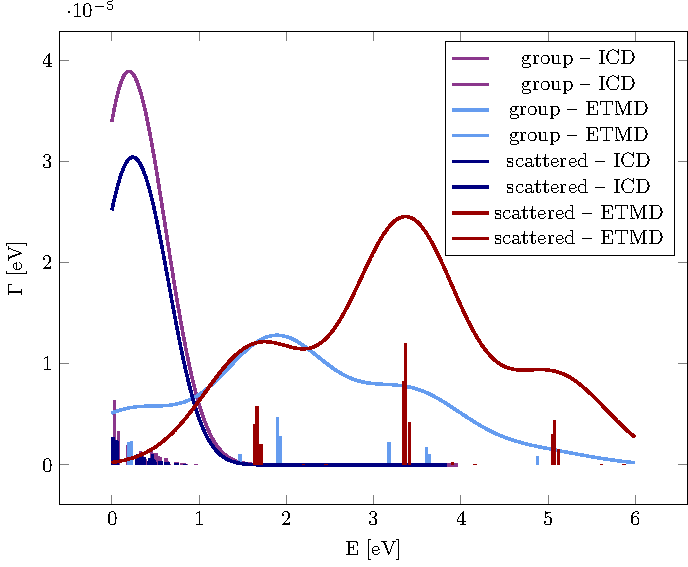
\includegraphics[width=8.5cm]{pics/ar_3_6in.pdf}
 \caption{Simulated ICD and ETMD electron spectra for clusters consisting of
          55 atoms out of which 6 are xenon atoms. These are either clustered
          (group) on one side of the cluster of evenly distributed
          inside the cluster (scattered). In both cases the ETMD peaks are
          clearly visible in the spectra.}
 \label{figure:ar_3_6in}
\end{figure}

For both cases the overall ICD spectra are very similar with concoluted
peaks at approximately \unit[0.3]{eV}. For the grouped xenon atoms ICD
signals at slightly higher energies are to be observed from ArXe pairs of
larger distances du to the different cluster structure. However, the
significant difference is to be observed in the ETMD3 spectra. The
interatomic xenon distance in the grouped xenon is shorther than in the
cluster with evenly distributed xenon atoms. Hence, the threefold
peak structure for the cluster with the grouped xenon atoms is seen at
lower ETMD3 electron energies than for the cluster with evenly
distributed xenon atoms. Additionally, the probabilty for an electron
transfer from a xenon to an argon atom decreases exponentially with the
interatomic distance. Therefore, only those xenon atoms which have argon
atoms as their direct neighbours have a significant contribution to the
total decay width and the total ETMD3 decay width for the structure with
the grouped xenon atoms is lower than the total ETMD3 decay width of
the structure with evenly distributed xenon atoms.


For comparison with the previous assumptions of a xenon core surrounded
by argon atoms we investigated 13 and 55 atoms clusters with one or two
xenon atoms in the core. Some of the corresponding
spectra are shown in Figure \ref{figure:xe_3_in}.

\begin{figure}[h]
 \centering
 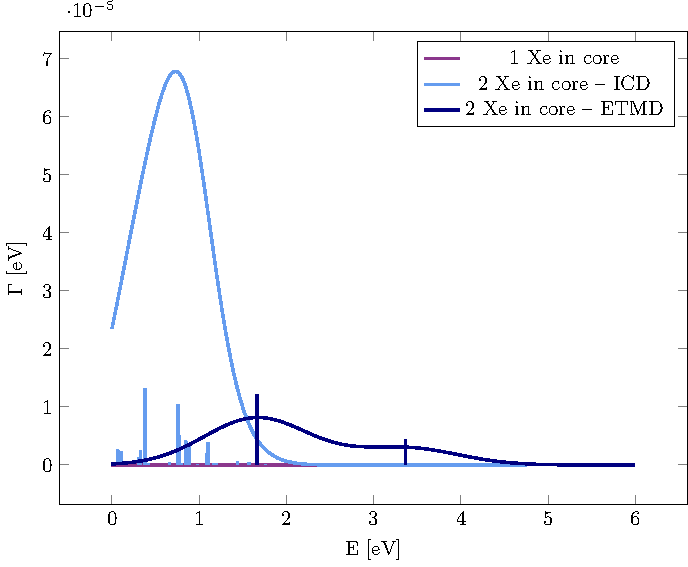
\includegraphics[width=8.5cm]{pics/xe_3_in.pdf}
 \caption{Simulated ICD and ETMD electron spectra for argon clusters with
          one or two atoms in the core of the cluster. In case of the xenon
          atom inhabiting the central position of the cluster for a 13 atoms
          cluster (not shown here) and a 55 atoms cluster all channels are closed
          for all pairs, which leads to no signal. For those clusters with two
          xenon atoms in the core the first ICD channel is open for some pairs
          and additionally ETMD is possible for multiple triples. Due to a
          different distance distribution compared to the clusters with an argon
          core the ICD peak is shifted to higher kinetic energies.}
 \label{figure:xe_3_in}
\end{figure}

For the clusters with only one xenon atom in the core and the ionization
energies used for the simulation of the secondary electron energies
all ICD channels are closed. Since the cluster contains only one xenon atom,
an ETMD3 is not possible. Hence there is no signal to be expected at all.
For a core consisting of two xenon atoms both an ICD and an ETMD3 spectrum
can be seen. Compared to the argon core cluster structures the ICD peak is
shifted to higher ICD electron energies not being in agreement with
the experimental spectrum. Additionally, the ICD and ETMD3 spectra overlap.
In case of the ETMD3 only three of the four different decay channels are
anergetically allowed.


Originally, very large argon-xenon clusters were measured experimentally,
which we approximate by a cluster consisting of 1415 xenon atoms surrounded
by two complete layers of argon atoms. The spectra are shown in Figure
\ref{figure:xe_8_lay1}.

\begin{figure}[h]
 \centering
 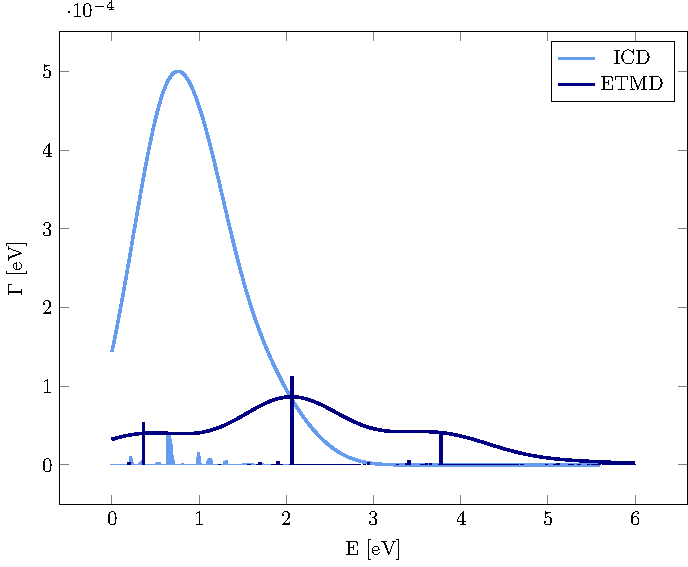
\includegraphics[width=8.5cm]{pics/xe_8_1lay.pdf}
 \caption{Simulated ICD and ETMD electron spectra for a large cluster consisting
          of a xenon core of 1415 atoms surrounded by two complete layers of
          argon atoms. The ICD and ETMD peak overlap such, that the peak structure
          might not be visible.}
 \label{figure:xe_8_lay1}
\end{figure}

Compared to the small clusters with a xenon core in Figure \ref{figure:xe_3_in}
the ICD peak is broadened and shifted to higher ICD electron energies which could be
expected due to the larger interatomic Ar-Xe distances in the large cluster and
the better stabilization of charges (the final state), which was taken care of
in the input of the simulation.
The ETMD3 peak is as well shifted to slightly higher energies allowing for the
fourth decay channel to open.

\section{Experimental Results}
\label{sec:exp_results}
%
%
\begin{table}
\caption{Properties of the outer valence spectra of mixed ArXe clusters. 
Spectra of pure Ar and Xe clusters are included for reference. 
All spectra were recorded at $h\nu = 17$~eV, except for the pure Xe clusters ($h\nu = 60$~eV). 
Binding energies $\EB$ were determined as the centre of gravity of the respective feature, while band width $w$ are the FWHM of a Gaussian fit. 
The average Xe content of the cluster ensemble, Xe$_{\rm cl}$, was determined from the areas of the respective photolines, corrected by their atomic photoionization cross sections (Ar 33.0 Mb, Xe 51.3 Mb)\cite{samson2002}.
Uncertainties are estimated as $\pm$3\,\% for the Xe content and 0.05~eV for the binding energies. 
The row labelled `(th.)' gives the binding energies used in the simulations of this paper, and the last row their atomic counterparts. 
Values for Ar 3p in the last row refer to the fine structure states.
\label{tab:valence}}
\begin{tabular}{ l c c c c c c c c}
%
\toprule
 \multicolumn{2}{r}{size} &  Xe$_{\rm in}$& $\EB$ (eV)& $w$ (eV)& \multicolumn{2}{c}{$\EB$ (eV)}  & $w$ (eV) &  Xe$_{\rm cl}$ \\
%
 \multicolumn{2}{r}{(label)}&  (\%) & Ar 3p & Ar 3p & Xe 5p$_{1/2}$ &  Xe 5p$_{3/2}$ & Xe 5p$_{3/2}$  &  (\%) \\
\midrule
% Ar, from Marko
 Ar & (1) &&  15.3  &  1.1 & & & &  \\
% Ar, from Marko 
 Ar & (2) &&  15.1  &  1.3 & & & &  \\
%
%  columns in the following: energies c.g. 51-plt-oval, widths Marko Diss., Xe content Marko Diss
% 1103 676, 679
 ArXe & S &1.2 & 15.36 & 0.9 & 13.07 & 11.75 & 0.85 & 12\\
% 1103 670
 ArXe & M &1.2 & 15.30 & 1.0 & 12.97 & 11.61 & 0.85 & 11\\
% 1103 671
 ArXe & L &1.2 & 15.25 & 1.1 & 12.91 & 11.52 & 1.08 & 10\\
% 1103 663
 ArXe & S &3.0 & 15.39 & 0.8 & 13.06 & 11.68 & 1.02 & 29\\
% 1103 640
 ArXe & M &5.0 & 15.31 & 0.6 & 12.96 & 11.44 & 1.24 & 53\\
% 0506 
 Xe &  & & & & 12.76 & 11.19 & 1.18 & 100\\
%
\midrule
%
%  1004  886  (UHe, c.g. + roi values)
 ArXe & XL &2.5 & 15.15 & 1.3 & 12.59 & 11.01 & 1.24 & 19\\
%
\midrule
% Date: Wed, 20 Jan 2016 11:27:39, From: Elke Fa?hauer <elke.fasshauer@uit.no>
 Ar, Xe & (th.) && 15.3 && 13.0 & 11.5 &&\\
%
 \multicolumn{2}{l}{(atomic)\cite{velchev,sansonetti}} && 15.76|15.94 && 13.43 & 12.13 &&\\
%
\bottomrule
\end{tabular}
\end{table}

\subsection{Outer valence spectra}
%
This section describes and discusses the outer valence spectra of the mixed Ar-Xe clusters. The main information we obtain from these spectra within the context of our theoretical considerations are the relative Xe contents in the mixed clusters (see Table\ \ref{tab:valence}). 
%
\begin{figure}[ht]
 \centering
 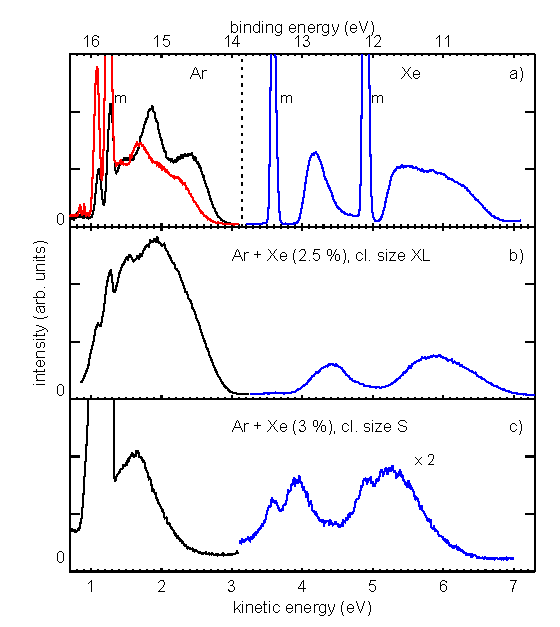
\includegraphics[width=8.5cm]{pics/figure_oval_1.pdf}
 \caption{
Outer valence photoelectron spectra of mixed Ar-Xe clusters, in comparison to the pure species. 
(a) shows the outer valence region of homogeneous Ar and Xe clusters, respectively (see text for details). 
The two lower panels show spectra of the mixed species with different mean size. 
Sharp lines marked `m' (for `monomer') result from photoionization of uncondensed atoms into the Ar 3p$_{1/2,3/2}$ and Xe 5p$_{1/2,3/2}$ final states. 
Labels in (b) and (c) give the Xe content in the expanding gas mixture (Xe$_{\rm in}$), which is lower than the Xe content observed in the heterogeneous clusters (Xe$_{\rm cl}$). 
The photon energy was 17~eV, apart from the pure Xe cluster spectrum (60 eV).
%{\color{red}{Die Stabilisierung der Xe-bulk Atome ist in den gemischten Cluster
% höher als in den gemischten Clustern. Das ist ungewöhnlich. Habt ihr hier
% verschiedene CLustergrößen?}}
}
 \label{figure:oval1}
\end{figure}


\begin{figure}[ht]
 \centering
 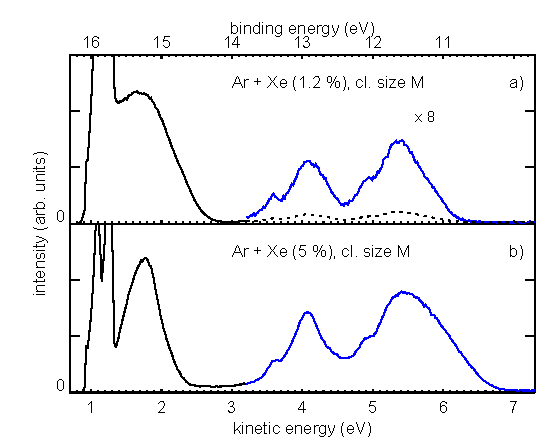
\includegraphics[width=8.5cm]{pics/figure_oval_2.pdf}
 \caption{
Outer valence photoelectron spectra of mixed Ar-Xe clusters from gas mixtures with different Xe concentration. 
For better visibility, a scaling factor is applied to the Xe part of the spectrum in panel (a).
See Figure \ref{figure:oval1} and text for details.
}
 \label{figure:oval2}
\end{figure}

Figure \ref{figure:oval1} shows the outer valence spectra of small and large ArXe clusters, compared to clusters of the pure gases. 
Qualitatively similar spectra have been published without detailed discussion in ref \citenum{lindblad}.
Differences are seen in particular for the Ar component. 
In pure Ar clusters, outer valence photoionization leads to a broad band, caused both by spin-orbit coupling and crystal field splitting. 
The relative importance of these two mechanisms remains under debate.\cite{hergenhahnprb,rolles,foerstel_arg1_2010} 
For larger clusters (e.g. $\langle N\rangle = 190$, black trace), the maximum at low binding energies becomes more pronounced, and is identified with emission from the cluster interior.\cite{hergenhahnprb,rolles}
At the particular photon energy selected here, atop of this band a sharp feature is also visible (in Figure \ref{figure:oval1} at a kinetic energy of about 1.8 eV).
For larger clusters (above $\langle N\rangle \approx 100$), over a range of photon energies of about 3 eV, its appararent binding energy changes in a way which is reminiscent to photoemission of crystalline bulk matter (`dispersion').\cite{foerstel_arg1_2010,foerstel_arg2_2011} 

Ar 3p spectra of the smaller mixed clusters (Figure \ref{figure:oval1}c, Figure \ref{figure:oval2}) show neither of these traits.
Rather, the Ar band is symmetric, less wide than in the pure clusters and at a higher binding energy.
Even for very large clusters (Figure \ref{figure:oval1}b) the asymmetry of the 3p band and the `dispersing feature' do not appear.
We characterize the spectral shape by giving a single value for the Ar 3p binding energy, and the FWHM of the feature.
Values for different expansion parameters, and for both Ar and Xe valence lines, are collected in Table\ \ref{tab:valence}.

We find experimentally that clusters we have produced have a Xe content Xe$_{\rm cl}$ between 10\,\% and 50\,\%.
A slight decrease of the binding energy with cluster size is seen for all outer valence lines, and is attributed to a larger final state polarization energy in larger clusters. 

For further interpretation of the shape of the Ar peaks we refer to photoemission spectra of condensed Ar monolayers, measured in several settings.\cite{jacobi,jacobi2}
Spectra were reported for physisorption of Ar on two different metal single crystal substrates, and for Ar atop of a Xe spacer layer adsorbed on the metal.
While the binding energy depends on the substrate, the spectral shape is very similar in all cases. 
Most spectra were recorded for emission along the surface normal, and show a double peak split by about 0.5 eV, leading to a structure with $w$ about 1 eV.
Although the splitting is larger than the gas phase fine structure split of 0.18 eV, the pertaining states have been assigned to Ar 3p$_{1/2}$ and 3p$_{3/2}$.
A crystal field splitting of the 3p$_{3/2}$ state has been assumed to be also present, but with a smaller value of 0.1-0.2 eV, approx.\cite{jacobi2} 
The spectrum clearly changes when going to an emission angle of 40$^\circ$ with respect to the surface normal (Figure 2 in ref \citenum{jacobi2}).
The higher binding energy peak significantly loses in intensity, and the spectrum is now dominated by a single peak comprising both crystal field split substates of Ar 3p$_{3/2}$, with a FWHM ($w$) of only 0.4 eV.
As our measured spectrum is comprised of contributions recorded under all emission angles with respect to the cluster surface, grazing emission will be the rule.
We therefore believe that the arguments given above make it plausible that only a single peak is observed in all our spectra.

Emission from the Xe 5p state shows a much larger fine structure splitting then from the Ar 3p state; it dominates the spectrum even in clusters (where other broadening mechanisms are also present).
The shift of the cluster bands with respect to the monomer lines in the largest mixed clusters we have probed (Figure \ref{figure:oval1}b) are similar to the ones in the pure Xe spectrum, the scaling law size of which is at somewhat more than five filled shells.
This indicates an approximate upper limit for the size of the Xe core in our mixed clusters, as their binding energy shift might be somewhat higher than the one in pure clusters, due to polarization of covering Ar layers.
Xe cluster features in the spectra of mixed clusters appear less asymmetric than the pure Xe spectrum, and also less asymmetric as some the ArXe spectra shown in ref \citenum{lindblad}.
This might be caused by the difference in photon energy ($h\nu = 90$ eV in ref \citenum{lindblad} and for the pure Xe spectrum, $h\nu = 32$ eV for the mixed ArXe spectra in this work).
% For the mixed clusters, the Xe band broadens and shifts towards lower binding energy for larger size clusters.
%For pure Xe clusters, an asymmetry observed in the Xe 5p$_{3/2}$ part has no counterpart in the respective spectra from the mixed clusters.
%This might be caused by the difference in photon energy, as can be seen from a comparison to literature spectra (ArXe at $h\nu = 90$ eV in ref \citenum{lindblad}, Xe at $h\nu = 20$ eV in ref \citenum{rolles}).
%For the largest clusters, the nominal size yielded from the jet parameters applied to a pure Xe expansion would correspond to clusters in which bulk atoms far outweigh those on the surface.
%At least for the 5p$_{1/2}$ photoelectron line, this would be seen as a clear asymmetry towards the low binding energy side, which is not observed in our spectra.


In Figure \ref{figure:oval2}, we compare the outer valence spectra of clusters with similar expansion conditions, but different composition of the gas mixture.
A Xe-rich mixture obviously leads to clusters with more intense Xe photolines, but besides that the main change consists in a narrowing of the Ar band.
A comparison with the Ar monomer features (clipped in the Figure) also shows an increased degree of condensation for the Ar gas in the expansion.

For the smallest clusters we have produced, a possible model is provided by calculated minimum energy structures of Ar$_N$Xe$_{38-N}$ (Figure 7 in ref \citenum{marques}).
We there see that for a Xe content of less than 60\,\%, core-shell systems are {\it not} formed, and although the Xe atoms tend to connect, the degree of Ar-Xe mixing is large.
While for low Xe content (approx. 10\,\%), some Ar atoms have only Ar nearest neighbours, for larger Xe content all Ar atoms seem to see both Ar and Xe nearest neighbours.
We believe this leads to the Ar 3p narrowing pointed out above.
For Figure \ref{figure:oval2}, possibly, some clusters of our ensemble already are in the core-shell regime, which would lead to an even lower 3p width.

For the largest clusters we have produced (Figure \ref{figure:oval1}b), the low binding energy of the Xe lines and the broadening of the Ar feature without appearance of the `bulk Ar'-maximum, supports formation of a Xe core covered by at least two layers of Ar.
If the scaling law size for a pure Ar expansion is taken as the lower limit for the cluster size, from the observed Xe content we arrive at clusters composed of a Xe core with four layers, covered by three layers of Ar (see Supporting Information).

Finally, comparing Figure \ref{figure:oval2} to Figure \ref{figure:oval1} reveals that much larger changes in the valence emission spectra occur by changes in size than by changes of the (relative) Xe content.
This finding is supported by the spectra shown in ref \citenum{lindblad}.
%
%
\subsection{Inner valence spectra}
%
We now focus on the Ar inner valence (3s) vacancy states. 
%
\begin{figure}[ht]
 \centering
 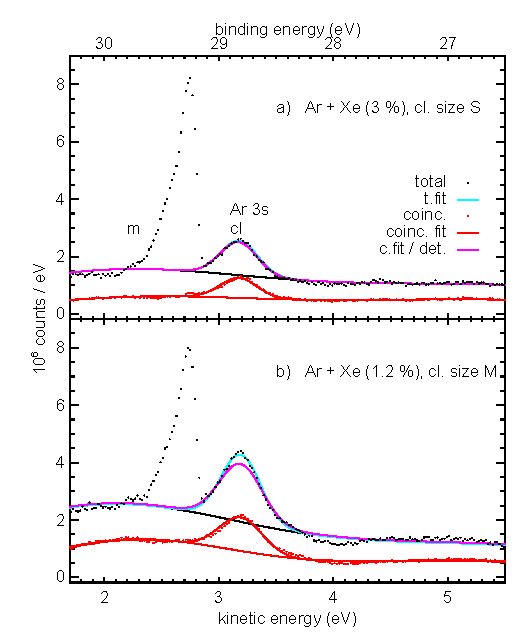
\includegraphics[width=8.8cm]{pics/figure_ival.pdf}
 \caption{
Photon excited electron spectra of mixed Ar-Xe clusters in the inner valence region.
Symbols show the Ar 3s photoline from clusters (`cl') and uncondensed Ar monomers (`m'), atop of a background resulting from inelastic intracluster scattering of outer valence photoelectrons (`excitonic satellites').\protect\cite{hergenhahn2002}
The photon energy was $h\nu = 32$ eV.
Panel (a) shows all electrons accumulated.
For the same conditions, in panel (b) we only show electrons that were detected in coincidence with a secondary electron of lower kinetic energy.
The black solid trace in (a), and red solid trace in (b) result from a least squares fit to the cluster part of the spectrum. 
The red solid trace in (a) is the fit shown in (b), divided by the detection efficiency of the spectrometer of 0.6.
Panels (c) and (d) show the same type of data for smaller clusters with a lower Xe content.
See text for details.
\label{figure:ival}
}
\end{figure}

Figure\ \ref{figure:ival} shows the Ar part of the inner valence spectrum for representative ArXe clusters. 
The total photoelectron signal looks similar to literature spectra for pure Ar clusters.\cite{feifel,zhang} 
A low energy tail seen for the Ar 3s monomer line results from the transmission properties of the electron spectrometer, together with the strongly positive angular distribution parameter of this line.\cite{zhang,kruit}
The Ar 3s cluster line shows no splitting into bulk and surface components, different to the literature on pure clusters but in agreement with our discussion of the outer valence spectra. 
The binding energy of the cluster line has values between 28.85 and 28.70 eV for all cluster ensembles with size label S-L, and 28.67 eV for the largest clusters measured. 
A small, but systematic decrease of the binding energy is observed when the cluster size is increased. 
The value assumed in the simulations is 28.7 eV.

If we produce a spectrum only from those electrons recorded as part of a two-electron coincidence (electron pair with kinetic energies ($e_1,e_2$)) the apparent intensity drops (compare panel b to a, and d to c in Figure \ref{figure:ival}).
This can partly be attributed to the finite detection efficiency of the spectrometer. 
Moreover, the monomer part of the Ar 3s signal completely disappears, as 3s photoionization of an uncondensed Ar atom in the gas jet cannot lead to emission of a second electron. 
Further features of these diagrams and the least squares fits shown in the Figure are discussed below.
%
%
\subsection{ICD/ETMD spectra}
%
\begin{figure}[ht]
 \centering
 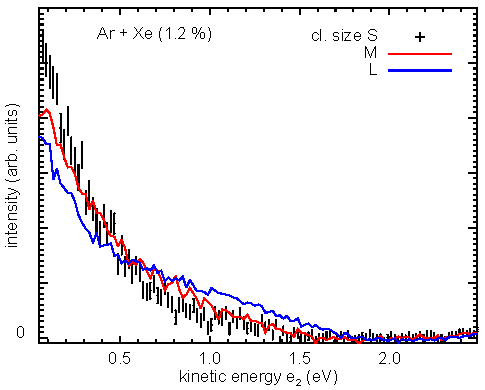
\includegraphics[width=8.5cm]{pics/figure_icd_12.pdf}
 \caption{
Energy spectrum of all coincident secondary (ICD or ETMD) electrons of kinetic energy $e_2$ pertaining to primary electrons of kinetic energy $e_1$ in the Ar 3s binding energy region. 
Spectra were recorded with a photon energy of $h\nu = 32$~eV. 
Black error bars show the data points for the smallest clusters measured (`S'), two larger clusters sizes are shown by the red and blue traces. 
Error bars for the latter are smaller than the ones shown and have been omitted.
For better comparison, all spectra are shown area-normalized. 
}
 \label{figure:icd_12}
\end{figure}
%
%
\begin{figure}[ht]
 \centering
 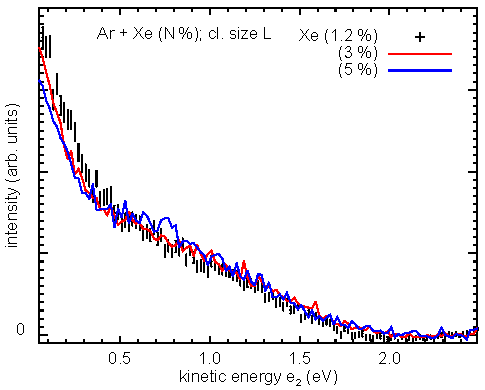
\includegraphics[width=8.5cm]{pics/figure_icd_l.pdf}
 \caption{
Energy spectrum of all coincident secondary (ICD or ETMD) electrons, kinetic energy $e_2$, for clusters of the same size, but from gas mixtures with different Xe concentration. See Figure \protect\ref{figure:icd_12} for details.
}
 \label{figure:icd_l}
\end{figure}
%
In Figure \ref{figure:icd_12}, we show the spectra of ICD/ETMD electrons pertaining to emission of an Ar 3s cluster photoelectron. 
Due to their low kinetic energy, without use of a coincidence method they could hardly be separated from the background of inelastically scattered photoelectrons.\cite{mucke}
This and the following Figure constitute the central experimental result of the article.
Spectra recorded at $h\nu = 34$ eV as a cross-check quantitatively agree to those shown here.
This underpins our assignment of this intensity to an autoionization process.
Further details on the data acquisition and analysis methodology, as well as the 34~eV spectra, are given in the Supporting Information.

Spectra for the three different cluster sizes in Figure \ref{figure:icd_12} are significantly different: Spectra for the larger clusters acquire more intensity in the 1-1.5 eV region and have less intensity for energies below 0.5 eV.
In contrast to that, the ICD/ETMD spectrum hardly varies when the composition of the expanding gas mixture, and with that the relative Xe content of the clusters, is changed (Figure \ref{figure:icd_l}).
The full set of ICD/ETMD spectra is shown as Supporting Information.

\begin{figure}[ht]
 \centering
 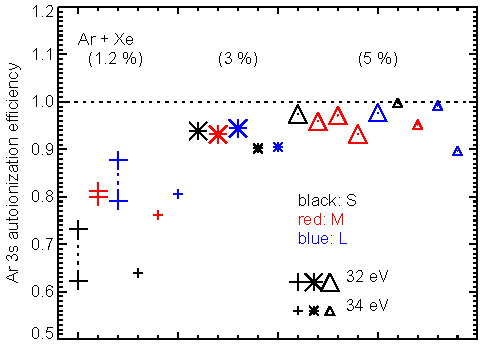
\includegraphics[width=8.5cm]{pics/figure_eff.pdf}
 \caption{
Efficiency of the decay of Ar 3s ionized states in ArXe clusters by emission of a secondary electron via ICD or ETMD. Values are arranged by Xe content of the initial gas mixture (`+' symbols: 1.2\,\%, asterisk: 3\,\%, triangle: 5\,\%). Symbol sizes indicate the photon energy (large symbols: 32 eV, small: 34 eV), and color indicates the cluster size (black symbols: S, red: M, blue: L). See text for details.
}
 \label{figure:eff}
\end{figure}
%
We now discuss which fraction of Ar 3s vacancy states relaxes via ICD or ETMD.
A method to derive this information has been established by some of us.\cite{foerstel_2013}
Briefly, we correct the intensity of the Ar 3s photoline in the coincident spectra by the detector efficiency, and divide it by the total (coincident and non-coincident) Ar 3s intensity.
The result gives the branching ratio of decay via ICD/ETMD vs. the sum of all channels, including those not involving electron emission.
(If all Ar 3s vacancies decay by emission of another electron, the coincident and non-coincident count rate differ only by the probability for the spectrometer to actually detect the secondary electron.
This figure has been determined as 0.6 for this data set, in the same way as discussed earlier.\cite{mucke_review})
To arrive at quantitative results, we have performed least squares fits of the non-coincident and coincident $e_1$ spectra.
The fits assumed one or two Gaussian peaks, resp., atop of a background modelled by two more Gaussian curves with very large widths.
The peak pertaining to the Ar 3s cluster photoline, with the background added, is shown by the black solid trace in Figure \ref{figure:ival}a and red solid trace in Figure \ref{figure:ival}b.
Moreover, the line labelled `c.fit/det.' shows the fit to the coincident events, corrected by the detection efficiency, and plotted atop of the non-coincident intensity. 
This virtually agrees with the fit to the total spectrum in Figure \ref{figure:ival}a, but not in \ref{figure:ival}c. 
The corresponding figure for the ICD/ETMD efficiency comes out as one for \ref{figure:ival}a, and significantly smaller than one for \ref{figure:ival}c.
Figure \ref{figure:eff} shows all results of this analysis.
The error in the autoionization efficiency shown is mainly determined by uncertainties in the peak/background separation.
%(Our choice for the background shape is shown in Figure \ref{figure:ival}.)
For the gas mixture with a Xe$_{\rm in}$ of 1.2\,\%, we therefore show results from fits using two different choices of the background shape in Figure \ref{figure:eff}.
Statistical errors are much smaller than the differences between the pairs of values arrived at such.

We found an Ar 3s autoionization efficiency which, for clusters with the lowest Xe content (Xe$_{\rm cl}$ approx. 10-12\,\%), is smaller than unity, and further decreases with decreasing cluster size. 
For larger Xe$_{\rm cl}$, the values are compatible with unity, within the accuracy of our experiment.

\section{Discussion}

We have discussed the experimental spectra in iSection \ref{} and
the expected features of spectra for different cluster types in
Section \ref{}. In this section we combine the experimental and theoretical
results in order to determine the structure of the noble gas clusters.


%\section{Discussion of Experimental Results}

\section{Summary}
%
We have presented comprehensive experimental and theoretical data for the
autoionization of inner valence ionized states in ArXe clusters.
Both ICD and ETMD are allowed for most cases we considered.
Because of energetical reasons ICD requires a separation of the final state
vacancies of \unit[7.58]{\AA} or more, which is about two times the typical
Ar-Xe distance.
We found that autoionization has an efficiency of 0.8 to 1.0 within the
experimental accuracy, that is it dominates over other modes of relaxation.
By comparing our measured spectra to calculations, we identified `long range'
ICD as the most important decay mode.


%%%%%%%%%%%%%%%%%%%%%%%%%%%%%%%%%%%%%%%%%%%%%%%%%%%%%%%%%%%%%%%%%%%%%
%% The "Acknowledgement" section can be given in all manuscript
%% classes.  This should be given within the "acknowledgement"
%% environment, which will make the correct section or running title.
%%%%%%%%%%%%%%%%%%%%%%%%%%%%%%%%%%%%%%%%%%%%%%%%%%%%%%%%%%%%%%%%%%%%%
\begin{acknowledgement}
%
We thank HZB for the allocation of synchrotron radiation beamtime, and the
Deutsche Forschungsgemeinschaft for funding via the Forschergruppe 1789.
E. F. gratefully acknowledges the Research
Council of Norway through a Centre of Excellence Grant (Grant No.\ 179568/V30)
for funding.
%
\end{acknowledgement}


%%%%%%%%%%%%%%%%%%%%%%%%%%%%%%%%%%%%%%%%%%%%%%%%%%%%%%%%%%%%%%%%%%%%%
%% The same is true for Supporting Information, which should use the
%% suppinfo environment.
%%%%%%%%%%%%%%%%%%%%%%%%%%%%%%%%%%%%%%%%%%%%%%%%%%%%%%%%%%%%%%%%%%%%%
%\begin{suppinfo}

%This will usually read something like: ``Experimental procedures and
%characterization data for all new compounds. The class will
%automatically add a sentence pointing to the information on-line:

%\end{suppinfo}

%%%%%%%%%%%%%%%%%%%%%%%%%%%%%%%%%%%%%%%%%%%%%%%%%%%%%%%%%%%%%%%%%%%%%
%% The appropriate \bibliography command should be placed here.
%% Notice that the class file automatically sets \bibliographystyle
%% and also names the section correctly.
%%%%%%%%%%%%%%%%%%%%%%%%%%%%%%%%%%%%%%%%%%%%%%%%%%%%%%%%%%%%%%%%%%%%%
\bibliography{arxe}

\end{document}
